\chapter{Implementacija i korisničko sučelje}
		
		
		\section{Korištene tehnologije i alati}
		
			%\textbf{\textit{dio 2. revizije}}
			
			% \textit{Detaljno navesti sve tehnologije i alate koji su primijenjeni pri izradi dokumentacije i aplikacije. Ukratko ih opisati, te navesti njihovo značenje i mjesto primjene. Za svaki navedeni alat i tehnologiju je potrebno \textbf{navesti internet poveznicu} gdje se mogu preuzeti ili više saznati o njima}.
			{Komunikacija unutar grupe najviše se odvijala preko aplikacije \underline{Discord}\footnote{\url{https://discord.com/}}, a manjim dijelom u početku putem Microsoftove platforme za poslovnu komunikaciju \underline{Teams}\footnote{\url{https://www.microsoft.com/hr-hr/microsoft-teams/}}. Za izradu gotovo svih UML dijagrama korišten je alat \underline{Astah UML}\footnote{\url{https://astah.net/products/astah-uml/}}, dok je dijagram baze podataka napravljen uz pomoć razvojnog okruženja \underline{DataGrip}\footnote{\url{https://www.jetbrains.com/datagrip/}} tvrtke JetBrains. Upravljanje različitim verzijama koda i dokumentacije obavljanno je uz pomoć sustava \underline{Git}\footnote{\url{https://git-scm.com/}}, a podatci su se čuvali u udaljenom repozitoriju na platformi \underline{GitLab}\footnote{\url{https://gitlab.com/}}.}
			
			{Članovi tima koji su izrađivali \textit{backend} koristili su \underline{IntelliJ IDEA}\footnote{\url{https://www.jetbrains.com/idea/}} ili \underline{Eclipse}\footnote{\url{https://www.eclipse.org/}} kao razvojno okruženje, dok su članovi na \textit{frontendu} koristili \textit{editor} \underline{Visual Studio Code}\footnote{\url{https://code.visualstudio.com/}}. IntelliJ i Eclipse su razvojna okruženja primarno namijenjena za razvoj softvera u Javi; Eclipseova funkcionalnost može se znatno proširiti \textit{plug-inovima}. Visual Studio Code jednostavan je uređivač izvornog koda koji se može koristiti s raznim programskim jezicima, a razvio ga je Microsoft.}
			
			{Za izradu \textit{backenda} aplikacije korišteni su radni okvir \underline{Spring Boot}\footnote{\url{https://spring.io/projects/spring-boot}} i jezik \underline{Java}\footnote{\url{https://www.java.com/}}. Spring Boot je specijalizacija radnog okvira \underline{Spring}\footnote{\url{https://spring.io/projects/spring-framework}} (ne nadomješta Spring) koja pojednostavljuje oblikovanje web aplikacije jer automatski konfigurira važne funkcionalnosti Springa. Na \textit{frontend} strani aplikacije korišteni su \underline{React}\footnote{\url{https://reactjs.org/}} i \underline{JavaScript}\footnote{\url{https://www.javascript.com/}}. React tehnički nije radni okvir, nego knjižnica pisana u JavaScriptu, iako se smatra jednim od najznačajnijih \textit{frontend} radnih okvira u vrijeme izrade ovog projekta.}
			
			{Za neke funkcionalnosti aplikacije korišteni su vanjski servisi: \underline{OpenStreetMap}\footnote{\url{https://www.openstreetmap.org}} za prikaz karte na kojoj se vide lokacije, \underline{OSRM}\footnote{\url{http://project-osrm.org/}}
			za računanje kartografovog puta do lokacije koju treba provjeriti i \underline{Cloudinary}\footnote{\url{https://cloudinary.com/}} za \textit{hostanje} slika lokacija i profilnih slika korisnika.}
			
			{Aplikacija je puštena u pogon na poslužitelju \underline{Heroku}\footnote{\url{https://www.heroku.com/}}, a baza podataka povezana je na Heroku preko \underline{Amazon AWS}\footnote{\url{https://aws.amazon.com/products/databases/}} usluge.}
			\eject 
		
	
		\section{Ispitivanje programskog rješenja}
			
%			\textbf{\textit{dio 2. revizije}}\\
%			
%			 \textit{U ovom poglavlju je potrebno opisati provedbu ispitivanja implementiranih funkcionalnosti na razini komponenti i na razini cijelog sustava s prikazom odabranih ispitnih slučajeva. Studenti trebaju ispitati temeljnu funkcionalnost i rubne uvjete.}
	
			
			\subsection{Ispitivanje komponenti}
%			\textit{Potrebno je provesti ispitivanje jedinica (engl. unit testing) nad razredima koji implementiraju temeljne funkcionalnosti. Razraditi \textbf{minimalno 6 ispitnih slučajeva} u kojima će se ispitati redovni slučajevi, rubni uvjeti te izazivanje pogreške (engl. exception throwing). Poželjno je stvoriti i ispitni slučaj koji koristi funkcionalnosti koje nisu implementirane. Potrebno je priložiti izvorni kôd svih ispitnih slučajeva te prikaz rezultata izvođenja ispita u razvojnom okruženju (prolaz/pad ispita). }

			{Ispitivanje komponenti provodimo pomoću JUnit javinog okvira za testiranje i pisanjem ispitnih slučajeva korištenjem jednog od javinih IDE, Eclipse ili IntelliJ.}
			
				\subsubsection {1. Ispitivanje traženja igrača korisničkim imenom}
				
					{Prilikom pisanja programskog koda za ovaj test koristi se anotacija \textit{@DataJpaTest} koji je specifičan za radni okvir \textit{spring} prilikom rada s \textit{Data Transfer Object} razredima. Očekivamo da će test biti uspješan i uspjeti pronaći igrača u bazi.}
					
						\begin{figure}[H]
							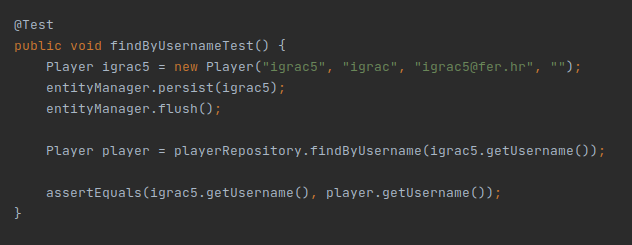
\includegraphics[width=\textwidth]{slike/playerFindByUsernameTest} 
							\centering
							\caption{Player Repository - JUnit, test}
							\label{}
						\end{figure}
					
				\subsubsection{Rezultat}
						
						\begin{figure}[H]
							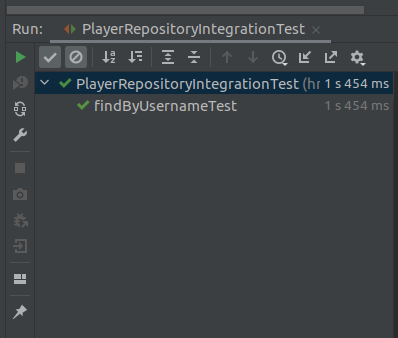
\includegraphics[width=\textwidth]{slike/playerFindByUsernameTest_result} 
							\centering
							\caption{Player Repository - JUnit, rezultat}
							\label{}
						\end{figure}
					
				\subsubsection {2. Ispitivanje traženja lokacije imenom}
				
					{Očekivamo da će test biti uspješan i uspjeti pronaći lokaciju u bazi.}
				
						\begin{figure}[H]
							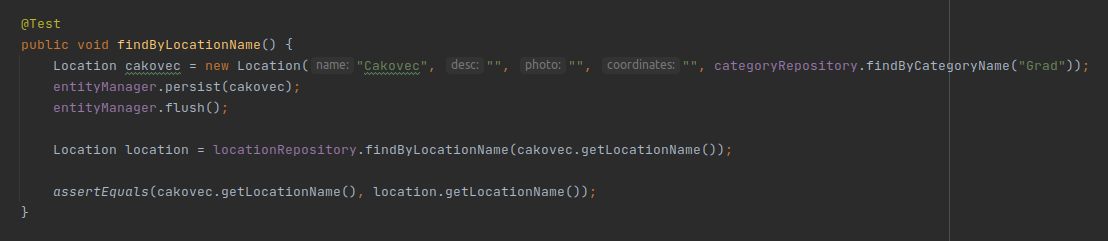
\includegraphics[width=\textwidth]{slike/locationFindByNameTest} 
							\centering
							\caption{Location Repository - JUnit, test}
							\label{}
						\end{figure}
					
				\subsubsection{Rezultat}
				
						\begin{figure}[H]
							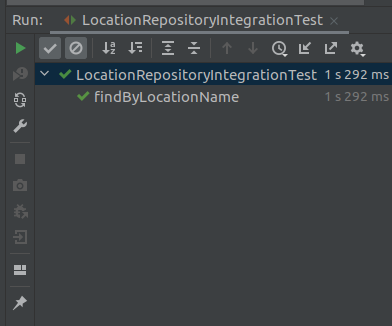
\includegraphics[width=\textwidth]{slike/locationFindByNameTest_result} 
							\centering
							\caption{Location Repository - JUnit, rezultat}
							\label{}
						\end{figure}
					
				\subsubsection {3. Ispitivanje traženja bespravnog zahtjeva za popis svih igrača}
					
					{Prilikom pisanja ovih testova koristi se anotacija \textit{@SpringBootTest} i \textit{@AutoConfigureMockMvc}. Očekivamo da će test biti uspješan jer se tijekom pretrage ne može obaviti provjera nad prijavljenim korisnikom kako bi se ustvrdilo da ima razinu adminstratorovih ovlasti.}
					
						\begin{figure}[H]
							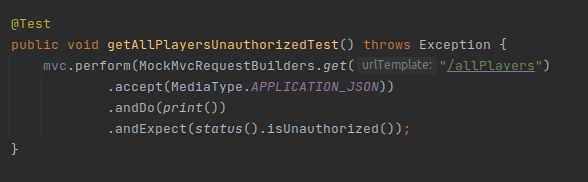
\includegraphics[width=\textwidth]{slike/unauthorizedTest} 
							\centering
							\caption{Admin Controller - JUnit, test}
							\label{}
						\end{figure}
					
				\subsubsection{Rezultat}
				
						\begin{figure}[H]
							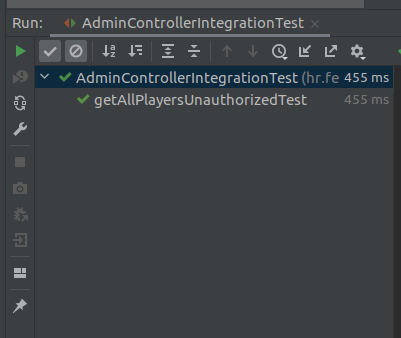
\includegraphics[width=\textwidth]{slike/unauthorizedTest_result} 
							\centering
							\caption{Admin Controller - JUnit, rezultat}
							\label{}
						\end{figure}
			
			\subsubsection {4. Ispitivanje razina ovlasti igrača i računanja udaljenosti}
			
				{Prilikom pisanja ovih testova koristi se anotacija \textit{@Mock} specifična za rad sa Service razredima. U ovom primjeru testiramo više metoda u razredu Player Service. Ispitujemo razine ovlasti kod postojećih igrača te metodu za računanje udaljenosti. Očekujemo da će za dane ulaze testovi proći.}
			
					\begin{figure}[H]
						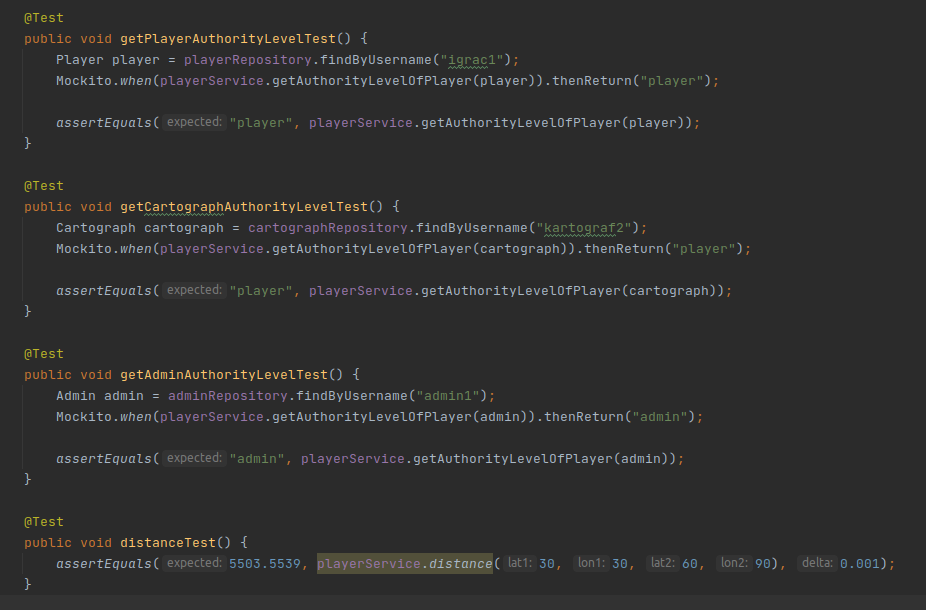
\includegraphics[width=\textwidth]{slike/playerServiceTest} 
						\centering
						\caption{Player Service - JUnit, test}
						\label{}
					\end{figure}
			
			\subsubsection{Rezultat}
			
					\begin{figure}[H]
						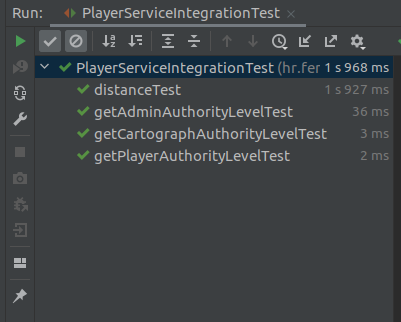
\includegraphics[width=\textwidth]{slike/playerServiceTest_result} 
						\centering
						\caption{Player Service - JUnit, rezultat}
						\label{}
					\end{figure}
			
			
			\eject
			
			\subsection{Ispitivanje sustava}
			
			% \textit{Potrebno je provesti i opisati ispitivanje sustava koristeći radni okvir Selenium\footnote{\url{https://www.seleniumhq.org/}}. Razraditi \textbf{minimalno 4 ispitna slučaja} u kojima će se ispitati redovni slučajevi, rubni uvjeti te poziv funkcionalnosti koja nije implementirana/izaziva pogrešku kako bi se vidjelo na koji način sustav reagira kada nešto nije u potpunosti ostvareno. Ispitni slučaj se treba sastojati od ulaza (npr. korisničko ime i lozinka), očekivanog izlaza ili rezultata, koraka ispitivanja i dobivenog izlaza ili rezultata.\\ }
			 
		%	 \textit{Izradu ispitnih slučajeva pomoću radnog okvira Selenium moguće je provesti pomoću jednog od sljedeća dva alata:}
		%	 \begin{itemize}
		%	 	\item \textit{dodatak za preglednik \textbf{Selenium IDE} - snimanje korisnikovih akcija radi automatskog ponavljanja ispita	}
		%	 	\item \textit{\textbf{Selenium WebDriver} - podrška za pisanje ispita u jezicima Java, C\#, PHP koristeći posebno programsko sučelje.}
		%	 \end{itemize}
		 %	\textit{Detalji o korištenju alata Selenium bit će prikazani na posebnom predavanju tijekom semestra.}
			
			{Ispitivanje sustava možemo provesti pomoću dodatka za preglednik Selenimu IDE i pisanjem ispitnih slučajeva korištenjem programskog sučelja, tj. mi koristimo Selenium WebDriver unutar JUnit testova. Pomoću dodatka za preglednik Selenium IDE snimaju se korisnikove akcije radi automatskog ponavljanja ispitnog slučaja.} 
			
			\subsubsection	{1. Ispitivanje dobre prijave na web aplikaciju GeoFighter }
			
				{Na ulazu unosimo podatke za prijavu već registriranog igrača (\emph{username: igrac1} i \emph{password: igrac}). Očekivani izlaz je preusmjeravanje na stranicu \emph{/home}. Preusmjeravanje pratimo prema elementima s određenih stranica. }
				
					\begin{figure}[H]
					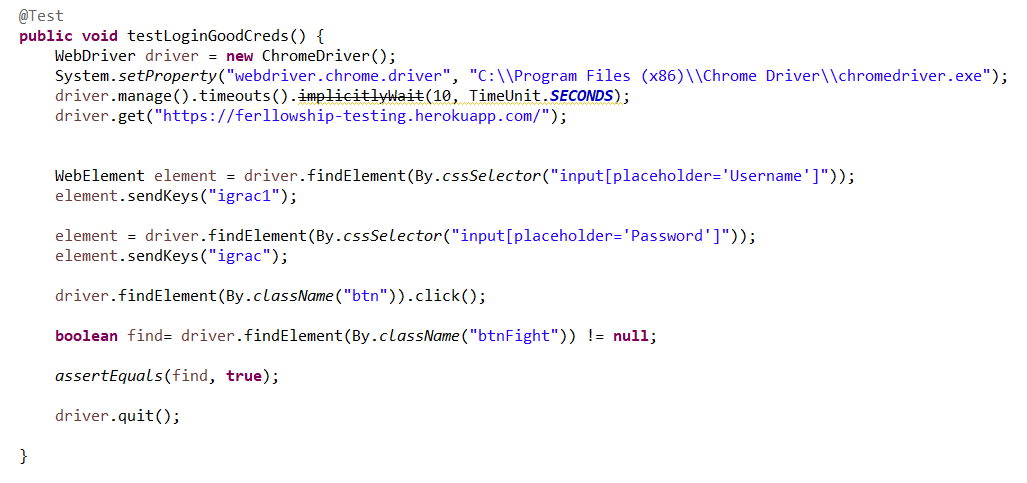
\includegraphics[width=\textwidth]{slike/JUSeTest1} 
					\centering
					\caption{Selenium WebDriver - JUnit, test1}
					\label{}
					\end{figure}
				
			\subsubsection{2. Ispitivanje loše prijave na web aplikaciju GeoFighter}
			
				{Na ulazu unosimo podatke za neregistriranog igrača (\emph{username: testadmin} i \emph{password: 22345}). Očekivani izlaz je ostanak na stranici za prijavu, što provjeravamo pomoću karakterističnih elemenata sa stranice.}
			
					\begin{figure}[H]
						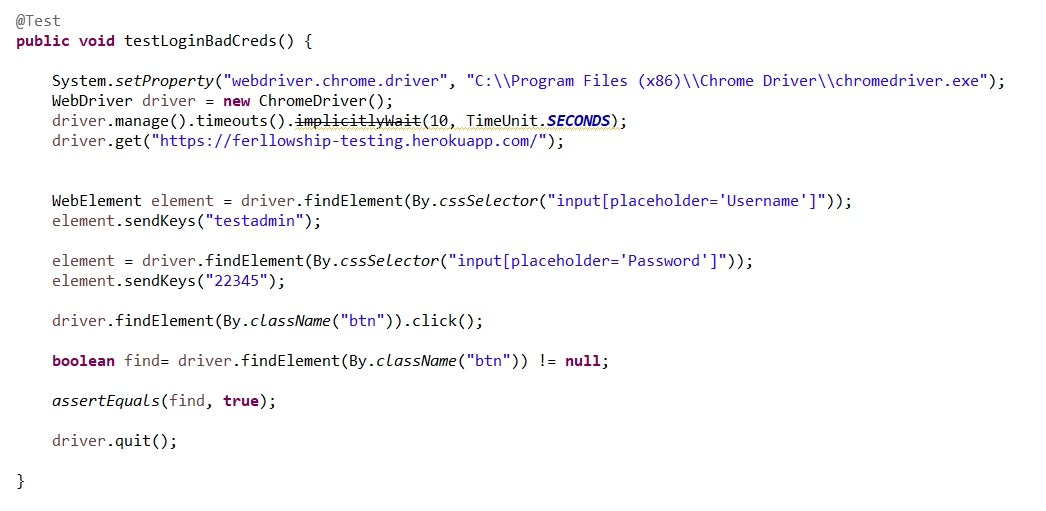
\includegraphics[width=\textwidth]{slike/JUSeTest2} 
						\centering
						\caption{Selenium WebDriver - JUnit, test2}
						\label{}
					\end{figure}
			
			\subsubsection{Rezultat}
			
				{Nakon pokretanja testova \emph{testLoginGoodCreds} i \emph{testLoginBadCreds}, dobili smo očekivani rezultat. Odnosno aplikacija je \textbf{prošla} testove.}
			
					\begin{figure}[H]
						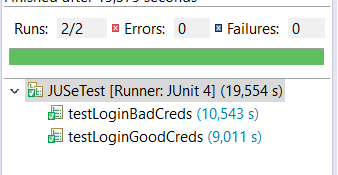
\includegraphics[width=\textwidth]{slike/rezultat_JUSeTest} 
						\centering
						\caption{Selenium WebDriver - JUnit, rezultat}
						\label{}
					\end{figure}
				
			\subsubsection{3. Ispitivanje postavljanja isključenja}
			
				{Ovo ispitvanje provodimo pomoću dodatka na Google Chrome \emph{Selenium IDE}. Prijavimo se kao \emph{admin1}, pregledamo profil \emph{igraca1}. Na ulazu testa unosimo trajno isključenje za \emph{igraca1} te se odjavimo kao \emph{admin1}. Očekivani izlaz je kad se pokušamo prijaviti kao \emph{igrac1} da nam to neće biti dozvoljeno dok će nam prijava kao \emph{igrac2} biti dozvoljena. Te radnje smo snimili pomoću Selenium IDE dodatka te ih pokrenuli s podatcima za \emph{igrac1}. Ako ponovno pokrenemo test i promijenimo korisničko ime na \emph{igrac2} vidimo da test dobro radi, odnosno s \emph{igrac2} smo se uspjeli prijaviti. Dobili smo željeni rezultat. Aplikacija je \textbf{prošla} test.}
					
					\begin{figure}[H]
						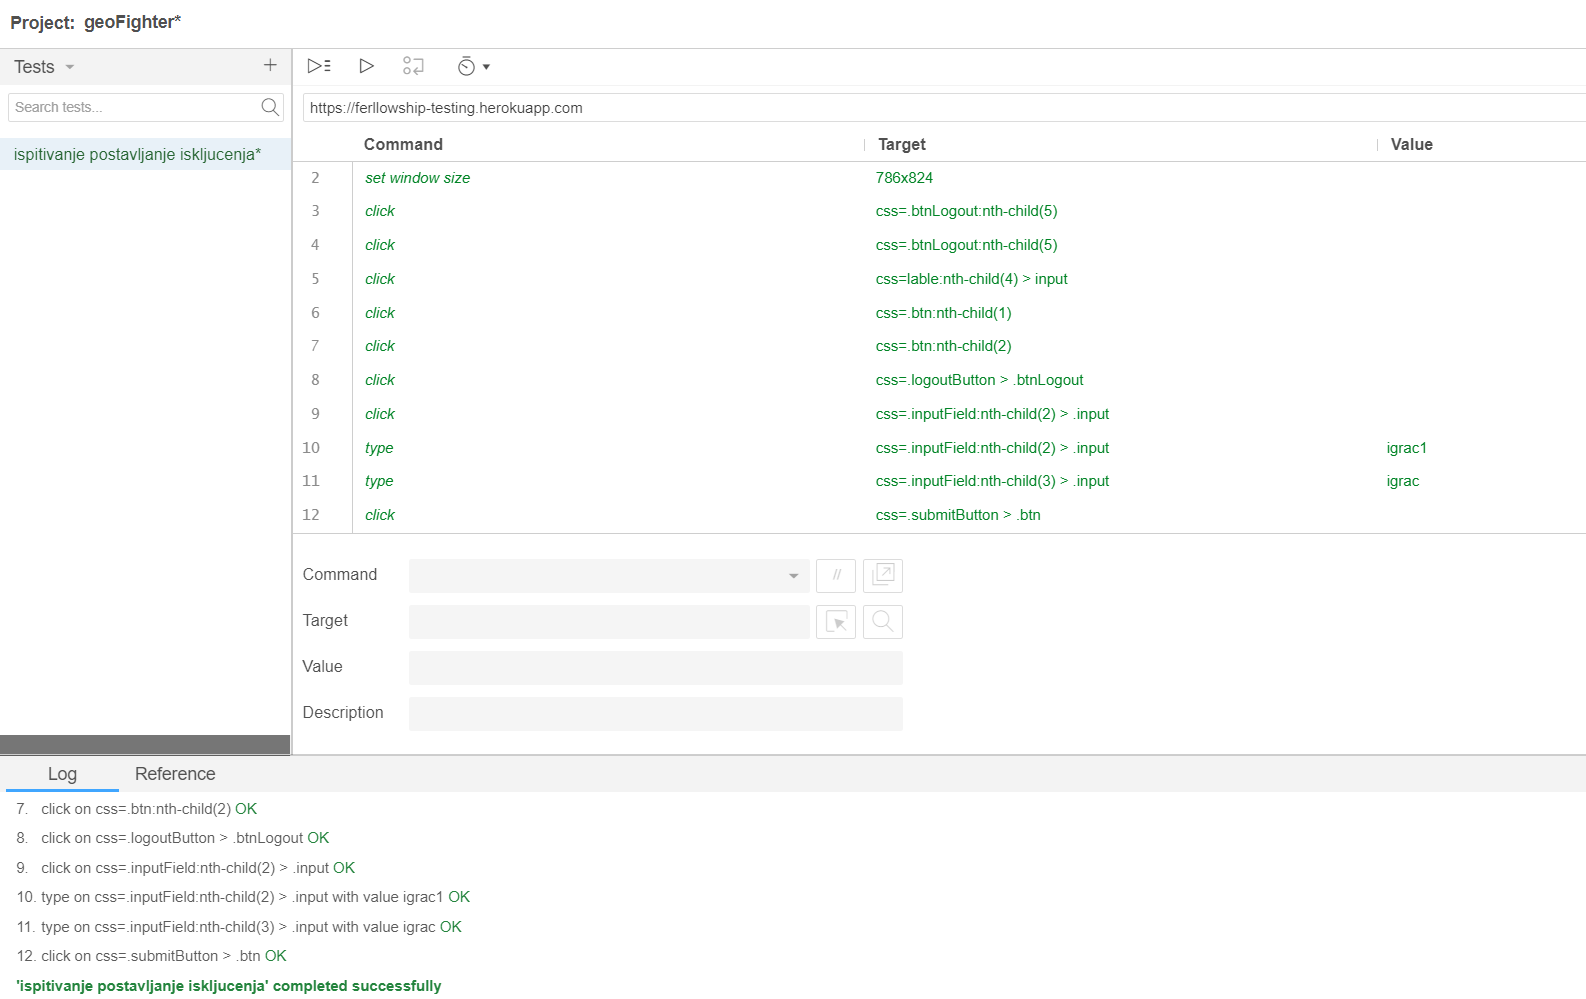
\includegraphics[width=\textwidth]{slike/SeleniumIDE_test1} 
						\centering
						\caption{Selenium IDE, ispitivanje postavljanja isključenja}
						\label{}
					\end{figure}
				\eject
			\subsubsection{4. Ispitivanje zahtjeva za kartografa}
			
				{Ovo ispitivanje provodimo pomoću dodatka na Google Chrome \emph{Selenium IDE}. Prijavimo se kao \emph{igrac1}. Na ulaz testa unosimo podatak za kartografa (IBAN i slika osobne iskazice). Očekivani izlaz je prikaz zahtjeva kod \emph{admin1}. Ove korake snimili smo pomoću Selenium IDE dodatka te smo dobili očekivani izlaz. Ukoliko u Selenium testu uklonimo jedan od podataka, željeni rezultat je da kod \emph{admin1} nema zahtjeva za kartografa. Nakon pokretanja testa vidimo da test dobro radi, odnosno da kod \emph{admin1} nema novih zahtjeva. Aplikacija je \textbf{prošla} test. }
					
					\begin{figure}[H]
						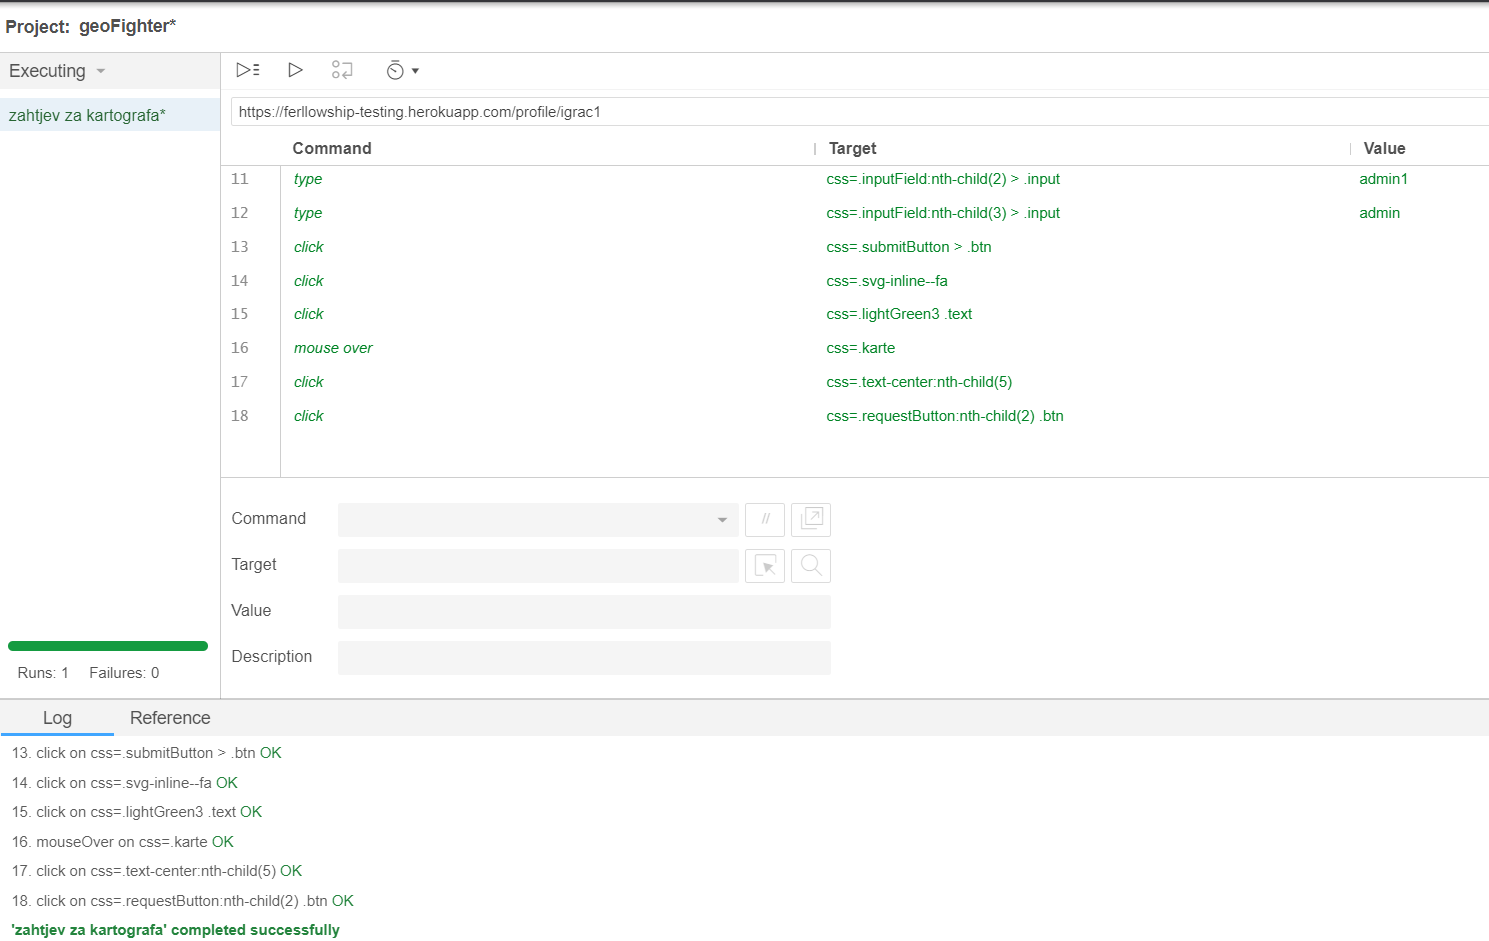
\includegraphics[width=\textwidth]{slike/SeleniumIDE_test2} 
						\centering
						\caption{Selenium IDE, ispitivanje zahtjeva za kartografa}
						\label{}
					\end{figure}
				
				
			\eject 
		
		
		\section{Dijagram razmještaja}
			
			%\textbf{\textit{dio 2. revizije}}
			
			 %\textit{Potrebno je umetnuti \textbf{specifikacijski} dijagram razmještaja i opisati ga. Moguće je umjesto specifikacijskog dijagrama razmještaja umetnuti dijagram razmještaja instanci, pod uvjetom da taj dijagram bolje opisuje neki važniji dio sustava.}
			
			{Dijagrami razmještaja (engl. deployment diagrams) opisuju topologiju skopovlja i programsku potporu koja se koristi u implementaciji sustava u njegovom radnom i produkcijskom okruženju. Dijagram razmještaja prikazuje razvijene aplikacije. Na poslužiteljskom računalu nalaze se web poslužitelj, poslužitelj baze podataka te poslužitelji Cloudinary i OSRM. Kako bi pristupili web aplikaciji, klijenti koriste web preglednik. Razmjena podataka između korisnika (igrač, kartograf, admin) i poslužitelja odvija se korištenjem HTTP protokola.}
			\begin{figure}[H]
				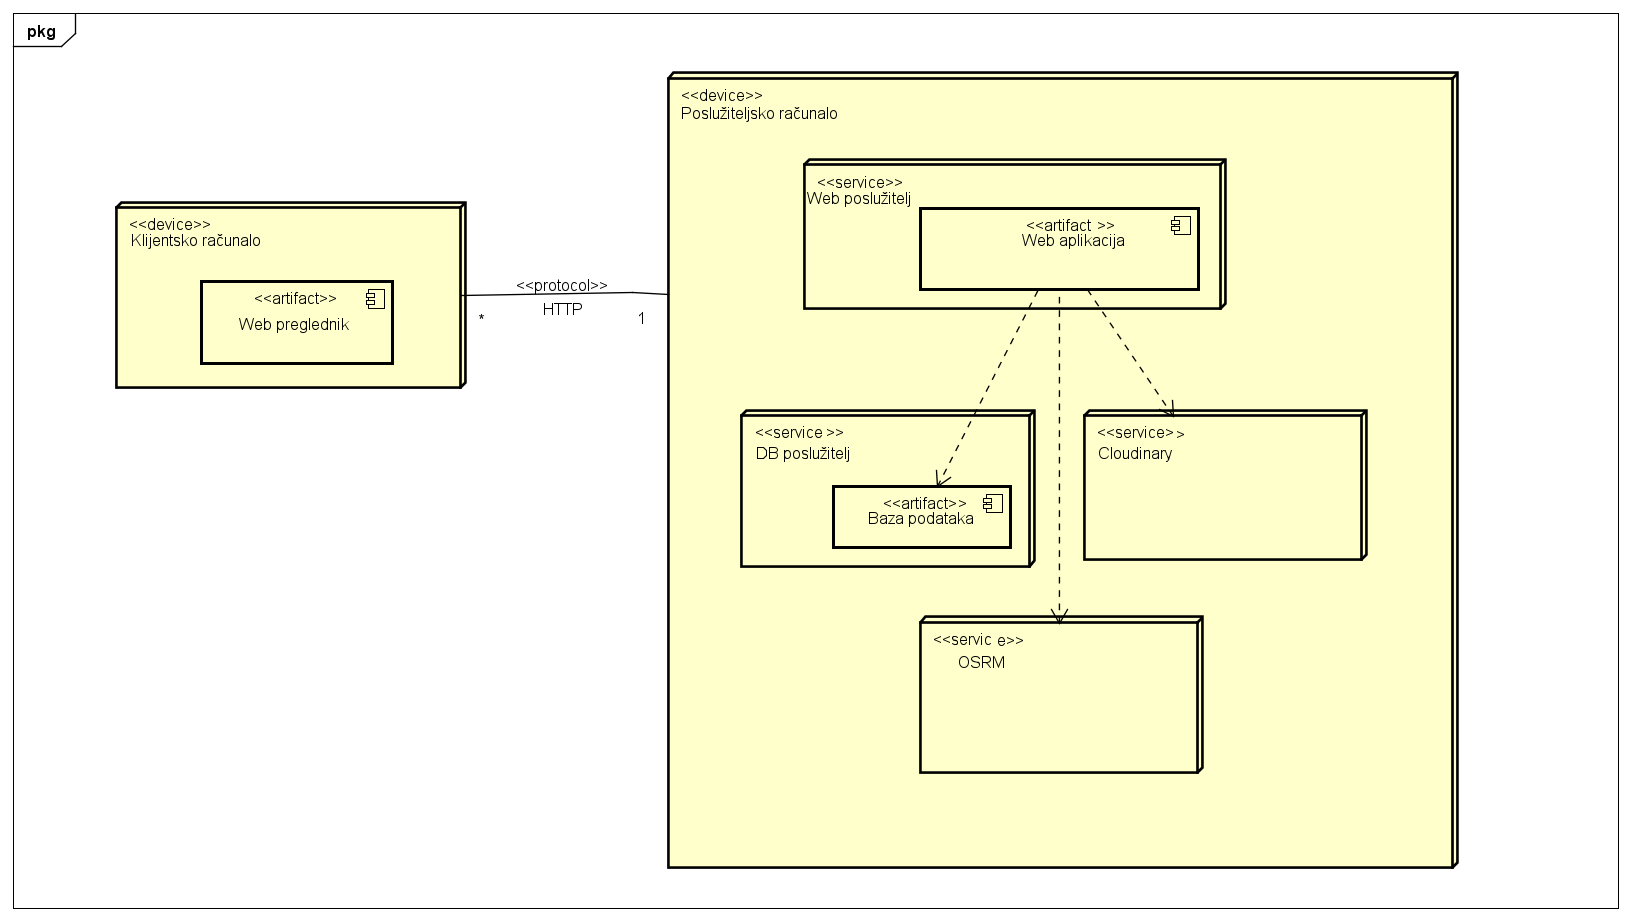
\includegraphics[width=\textwidth]{dijagrami/dijagram_razmjestaja} 
				\centering
				\caption{Dijagram razmještaja}
				\label{}
			\end{figure}
			\eject 
		
		\section{Upute za puštanje u pogon}
		
			\textbf{\textit{dio 2. revizije}}\\
		
			 \textit{U ovom poglavlju potrebno je dati upute za puštanje u pogon (engl. deployment) ostvarene aplikacije. Na primjer, za web aplikacije, opisati postupak kojim se od izvornog kôda dolazi do potpuno postavljene baze podataka i poslužitelja koji odgovara na upite korisnika. Za mobilnu aplikaciju, postupak kojim se aplikacija izgradi, te postavi na neku od trgovina. Za stolnu (engl. desktop) aplikaciju, postupak kojim se aplikacija instalira na računalo. Ukoliko mobilne i stolne aplikacije komuniciraju s poslužiteljem i/ili bazom podataka, opisati i postupak njihovog postavljanja. Pri izradi uputa preporučuje se \textbf{naglasiti korake instalacije uporabom natuknica} te koristiti što je više moguće \textbf{slike ekrana} (engl. screenshots) kako bi upute bile jasne i jednostavne za slijediti.}
			
			
			 \textit{Dovršenu aplikaciju potrebno je pokrenuti na javno dostupnom poslužitelju. Studentima se preporuča korištenje neke od sljedećih besplatnih usluga: \href{https://aws.amazon.com/}{Amazon AWS}, \href{https://azure.microsoft.com/en-us/}{Microsoft Azure} ili \href{https://www.heroku.com/}{Heroku}. Mobilne aplikacije trebaju biti objavljene na F-Droid, Google Play ili Amazon App trgovini.}
			
			
			\eject 